\documentclass{article}

% Language setting
% Replace `english' with e.g. `spanish' to change the document language
\usepackage[english]{babel}
\usepackage{float}

% Set page size and margins
% Replace `letterpaper' with `a4paper' for UK/EU standard size
\usepackage[letterpaper,top=2cm,bottom=2cm,left=3cm,right=3cm,marginparwidth=1.75cm]{geometry}

% Useful packages
\usepackage{amsmath}
\usepackage{graphicx}
\usepackage[colorlinks=true, allcolors=blue]{hyperref}

\title{Labwork 3: Logistic Regression}
\author{Nguyen Nhu Duy - 2540044}

\begin{document}
\setlength{\parindent}{0pt}
\maketitle
\section{Implement the algorithm}
\textbf{Step 1:} Define the sigmoid function, the prediction function \(f(x)\), and the logistic loss function \(L(x)\). Then, compute the partial derivatives of the loss function with respect to the weights \(w_0\), \(w_1\), and \(w_2\).

\textbf{Step 2:} Randomly initialize the weights \(w_0, w_1, w_2\). Define the learning rate \(r\) and the stopping threshold for the loss value.

\textbf{Step 3:} Perform gradient descent using the following iterative process:

\begin{itemize}
    \item Compute the gradients of the loss function for all training samples.
    
    \item Update the weights:
    \[
    w = w - r \times \frac{\partial L}{\partial w}
    \]
    
    \item Recompute the average loss value.
    
    \item Stop when the loss is smaller than the threshold; otherwise, repeat the process.
\end{itemize}

Finally, the optimized weights are used to make predictions for the dataset.

\section{Effect of different learning rate r}

\begin{table}[h]
\centering
\begin{tabular}{|c|c|}
\hline
Learning Rate & Iterations  \\
\hline
0.7 & Not converge \\
0.6 & 2713 \\
0.5 & 4453 \\
0.1 & 25597  \\
0.01 & 257465 \\
\hline
\end{tabular}
\caption{Effect of different learning rates with threshold = 0.2}
\end{table}

The results in Table 1 show that the learning rate has a significant impact on the convergence speed of gradient descent. 

When the learning rate is too small, such as \(r = 0.01\) or \(r = 0.1\), the algorithm converges very slowly and requires a large number of iterations to reach the stopping threshold. On the other hand, when the learning rate is too large, such as \(r = 0.7\), the algorithm becomes unstable and fails to converge because the updates overshoot the minimum point.

The experimental results indicate that learning rates between \(0.5\) and \(0.6\) provide the best performance. In this range, the algorithm converges much faster while still maintaining stable optimization. Therefore, choosing an appropriate learning rate is important to balance convergence speed and stability in gradient descent.

\section{Results visualization}

\begin{figure}[H]
    \centering
    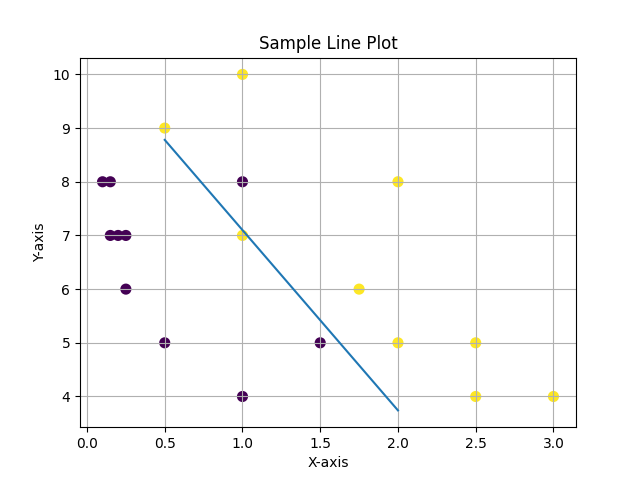
\includegraphics[width=0.5\linewidth]{plot_data.png}
    \caption{Plot the data point and Decision Line}
\end{figure}

The figure illustrates the distribution of the data points along with the learned decision boundary produced by logistic regression. The downward-sloping line separates the two classes, showing that the model successfully learned a linear classification boundary.


\section{Conclusion}

In this labwork, logistic regression was implemented using gradient descent optimization. The experiment demonstrated that the learning rate strongly affects the convergence behavior of the algorithm. Small learning rates lead to slow convergence, while excessively large learning rates may cause instability and divergence. The results show that choosing an appropriate learning rate is essential for efficient and stable optimization.

\end{document}